
%%%%%%%%%%%%%%%%%%%%%%%%%%%%%%%%%%%%%%%%%%%%%%%%%%%%%%%%%%%%%%%%%%%%%%%%%%%%%%%%%%%%%%%
%%%%%%%%%%%%%%%%%%%%%%%%%%%%%%%%%%%%%%%%%%%%%%%%%%%%%%%%%%%%%%%%%%%%%%%%%%%%%%%%%%%%%%%
% 
% This top part of the document is called the 'preamble'.  Modify it with caution!
%
% The real document starts below where it says 'The main document starts here'.

\documentclass[12pt]{article}

\usepackage{amssymb,amsmath,amsthm}
\usepackage[top=1in, bottom=1in, left=1.25in, right=1.25in]{geometry}
\usepackage{fancyhdr}
\usepackage{enumerate}
\usepackage{listings}
\usepackage{graphicx}
\usepackage{float}
\usepackage{multicol}
% Comment the following line to use TeX's default font of Computer Modern.
\usepackage{times,txfonts}
\usepackage{mwe}
\usepackage{caption}
\usepackage{subcaption}




\makeatletter
\renewcommand*\env@matrix[1][*\c@MaxMatrixCols c]{%
  \hskip -\arraycolsep
  \let\@ifnextchar\new@ifnextchar
  \array{#1}}
\makeatother

\newtheoremstyle{homework}% name of the style to be used
  {18pt}% measure of space to leave above the theorem. E.g.: 3pt
  {12pt}% measure of space to leave below the theorem. E.g.: 3pt
  {}% name of font to use in the body of the theorem
  {}% measure of space to indent
  {\bfseries}% name of head font
  {:}% punctuation between head and body
  {2ex}% space after theorem head; " " = normal interword space
  {}% Manually specify head
\theoremstyle{homework} 

% Set up an Exercise environment and a Solution label.
\newtheorem*{exercisecore}{Exercise \@currentlabel}
\newenvironment{exercise}[1]
{\def\@currentlabel{#1}\exercisecore}
{\endexercisecore}

\newcommand{\localhead}[1]{\par\smallskip\noindent\textbf{#1}\nobreak\\}%
\newcommand\solution{\localhead{Solution:}}

%%%%%%%%%%%%%%%%%%%%%%%%%%%%%%%%%%%%%%%%%%%%%%%%%%%%%%%%%%%%%%%%%%%%%%%%
%
% Stuff for getting the name/document date/title across the header
\makeatletter
\RequirePackage{fancyhdr}
\pagestyle{fancy}
\fancyfoot[C]{\ifnum \value{page} > 1\relax\thepage\fi}
\fancyhead[L]{\ifx\@doclabel\@empty\else\@doclabel\fi}
\fancyhead[C]{\ifx\@docdate\@empty\else\@docdate\fi}
\fancyhead[R]{\ifx\@docauthor\@empty\else\@docauthor\fi}
\headheight 15pt

\def\doclabel#1{\gdef\@doclabel{#1}}
\doclabel{Use {\tt\textbackslash doclabel\{MY LABEL\}}.}
\def\docdate#1{\gdef\@docdate{#1}}
\docdate{Use {\tt\textbackslash docdate\{MY DATE\}}.}
\def\docauthor#1{\gdef\@docauthor{#1}}
\docauthor{Use {\tt\textbackslash docauthor\{MY NAME\}}.}
\makeatother

% Shortcuts for blackboard bold number sets (reals, integers, etc.)
\newcommand{\Reals}{\ensuremath{\mathbb R}}
\newcommand{\Nats}{\ensuremath{\mathbb N}}
\newcommand{\Ints}{\ensuremath{\mathbb Z}}
\newcommand{\Rats}{\ensuremath{\mathbb Q}}
\newcommand{\Cplx}{\ensuremath{\mathbb C}}
%% Some equivalents that some people may prefer.
\let\RR\Reals
\let\NN\Nats
\let\II\Ints
\let\CC\Cplx

%%%%%%%%%%%%%%%%%%%%%%%%%%%%%%%%%%%%%%%%%%%%%%%%%%%%%%%%%%%%%%%%%%%%%%%%%%%%%%%%%%%%%%%
%%%%%%%%%%%%%%%%%%%%%%%%%%%%%%%%%%%%%%%%%%%%%%%%%%%%%%%%%%%%%%%%%%%%%%%%%%%%%%%%%%%%%%%
% 
% The main document start here.

% The following commands set up the material that appears in the header.
\doclabel{Math 614: Homework 6}
\docauthor{Stefano Fochesatto}
\docdate{\today}


\begin{document}


\begin{exercise}{P14} Equation 10.1 on page 77 is a cartoon of how Householder triagularization works on a 
  5x3 matrix. Turn this cartoon into a specific calculation by showing the stages $A$, $Q_1A$, 
  $Q_2Q_1A$, and $Q_3Q_2Q_1A = R$ on the following matrix: 
  \begin{equation*}
    A = 
    \begin{bmatrix}
      1 &2 & 3 \\
      2 &0 & -2 \\
      1 &3 & 5\\ 
      4 &5 & 6\\
      3 &-3& 3 
    \end{bmatrix}
  \end{equation*}
  \solution First we need to construct the first Householder reflector $F_1$. Recall equation 10.4 and note that geometrically we 
  want $v = ||x||e_1 - x$ for each $x$ pulled from $A$, 
  \begin{equation*}
    F = I - 2\dfrac{vv^*}{v^*v}.
  \end{equation*}
  To construct each unitary recall equation 10.2 and we get, 
  \begin{equation*}
    Q_k = \begin{bmatrix}
      I & 0\\
      0 & F
    \end{bmatrix}.
  \end{equation*}
  Consider the following MATLAB script which computes each unitary $Q_i$ and stores them in a Matlab cell,\\ 
  \textbf{Code:}
  \begin{center}
    \lstinputlisting[basicstyle = \small]{P16.m}
  \end{center} 
  \textbf{Console:}
  \begin{center}
    \lstinputlisting[basicstyle = \small]{r2.txt}
  \end{center} 
\end{exercise}
\vspace{1in}





\begin{exercise}{P15} The matlab built-in qr() computes the $QR$ factorization using Householder transformations as 
  described in lecture 10. This problem asks you to go ahead and use it! The purpose of this problem, is to 
  show that $QR$ had a completely different purpose.\\
  \begin{enumerate}
    \item[a.] By searching for 'Unsolvable quintic polynomials, ' for example, confirm that there is a theorem which shows that 
    fifth and higher-degree polynomials cannot be solved using finitely many operations including roots. In other words, there is 
    no finite formula for the roots of such polynomials. Who proved this theorem and when? Show a quintic polynomials for which it is know that 
    there is no finite formula. 
    \solution The theorem regarding the solvability of quintic polynomials goes as follows: 'there exists no solution in radicals to general 
    polynomial equations of degree five or higher with arbitrary coefficients. From what I was 
    able to find online the theorem is called the Abel-Ruffini theorem and apparently it first appeared in Paolo Ruffini's \emph{Teorie generale delle equazioni} 
    in 1799. In 1824 Norwegian mathematician Niels Henrik Abel would go on to produce a more rigorous proof of the theorem. Later Evariste Galois would go on to prove 
    a more generalized form of the theorem (I'd need to do some more reading before going into further detail) but died in a duel before publishing any of his work. Galois' work
    showed that $x^5 - x - 1 = 0$ was the simplest polynomial which cannot be solved using finitely many operations.\\
    \vspace{.15in}
    
    
    \item[b.] At the Matlab/Octave command line, try the following\dots\\
    \textbf{Console:}
    \begin{center}
      \lstinputlisting[basicstyle = \small]{r2.txt}
    \end{center} 
  \end{enumerate}
  We can see that as we increase the number of iterations the value of $A_i$ converges to the eigenvalue matrix of 
  $A$.
  %%%%%%%%%%%%%%% Do a little bit more
  \vspace{.15in}

  \item[c. ] Too see a bit more of what is going on in part $(b.)$ show that 
  \begin{equation*}
    A_{i+1} = Q_i^*A_iQ_i. 
  \end{equation*}  
  This shows that $A_{i+1}$ and $A_i$ have the same eigenvalues, explain.\\
  \solution First consider the $QR$ decomposition of $A_i$, and note that, 
  \begin{equation*}
    A_i = Q_iR_i
  \end{equation*}
  Know left multiply by $Q_i^*$ and right multiply by $Q_i$ to get, 
  \begin{equation*}
    Q_i^*A_iQ_i =  Q_i^*Q_iR_iQ_i  = R_iQ_i. 
  \end{equation*}
  Applying our definition of $A_{i+1}$ we get, 
  \begin{equation*}
    Q_i^*A_iQ_i  = A_{i+1}. 
  \end{equation*}
  To show that $A_{i+1}$ and $A_i$ have the same eigenvalues, let's suppose the eigenvalue 
  decomposition of $A_i = X^{-1} \Lambda X$. By substitution into our last equation we get, 
    \begin{equation*}
      Q_i^*X^{-1} \Lambda XQ_i  = A_{i+1}.  
  \end{equation*}
  Let $Y = Q_i^*X^{-1}$ and note that, 
  \begin{equation*}
    Y^{-1} = (Q_i^*X^{-1})^{-1} = X^{-1^{-1}}Q_i^{*^{-1}} =  XQ_i.
  \end{equation*}
  Thus we get the following, 
  \begin{equation*}
   Y \Lambda Y^{-1} = A_{i+1}.  
  \end{equation*}
  Therefore $A_{i+1}$ must have the same eigenvalues as $A_i$.
  \vspace{.15in}


  \item[d. ] Write a few sentences which relate parts a and b. \\
  \solution What we want to highlight here is the relationship between polynomial root finding 
  and eigenvalue problems. When we computed eigenvalues by-hand it involved creating the characteristic 
  equation for a matrix, and solving for the roots of that polynomial gave us the eigenvalues. Part a shows us that 
  there is no way to compute the roots of a quintic polynomial using exact arithmetic, and therefore there is no way of 
  computing the eigenvalues of a rank 5 matrix. Part b shows us an iterative method for solving eigenvalue problems.
  Note that by back-substituting the recurrence relation in part a (with some matrix algebra) we get to product described in 
  $25.4$ of lecture 25. \\
  
\end{exercise}

\vspace{1in}





\begin{exercise}{P16} Either by using the built in funciton polyfit() and polyval(), or by setting up linear systems
  and solving using Matlab's backslash command, reproduce Figures 11.1 and 11.2.\\
  \solution  Consider the following matlab code.\\
  \textbf{Code:}
  \begin{center}
    \lstinputlisting[basicstyle = \small]{r10.txt}
  \end{center} 
  \begin{figure}[H]
    \begin{center}
    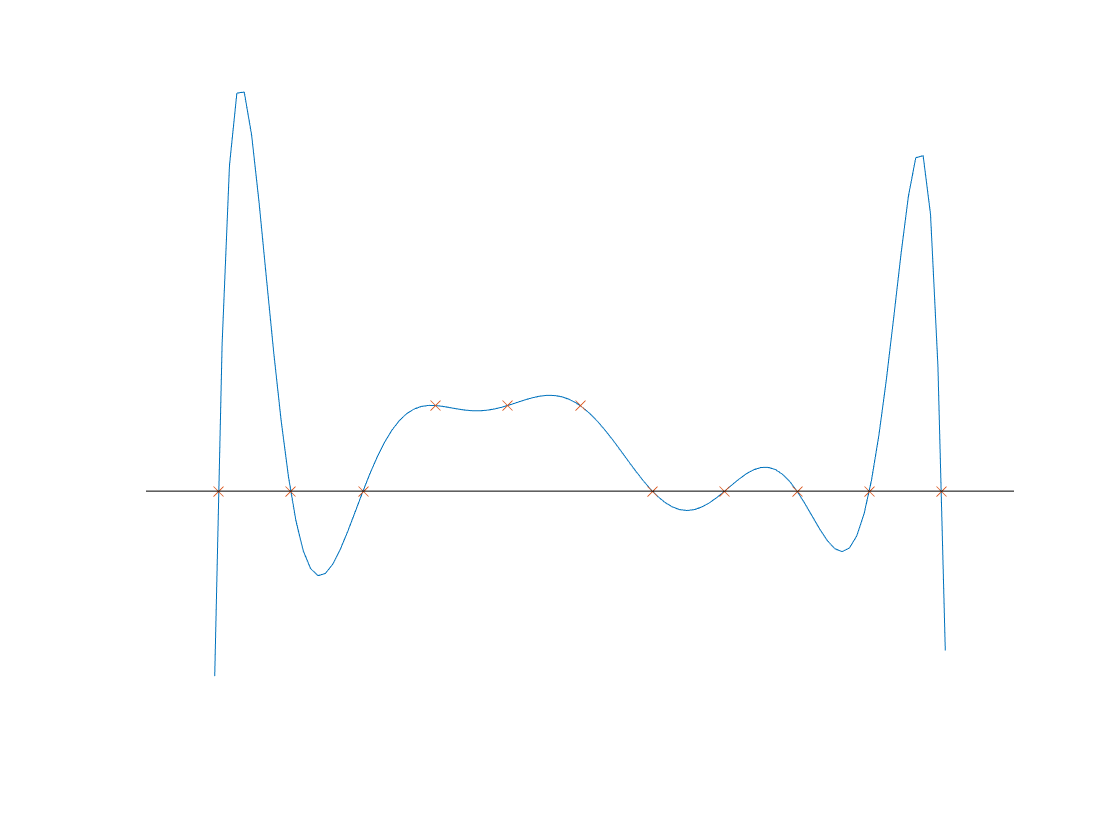
\includegraphics[width = \textwidth]{plot2.png}
    \end{center}
  \end{figure}
  \begin{figure}[H]
    \begin{center}
    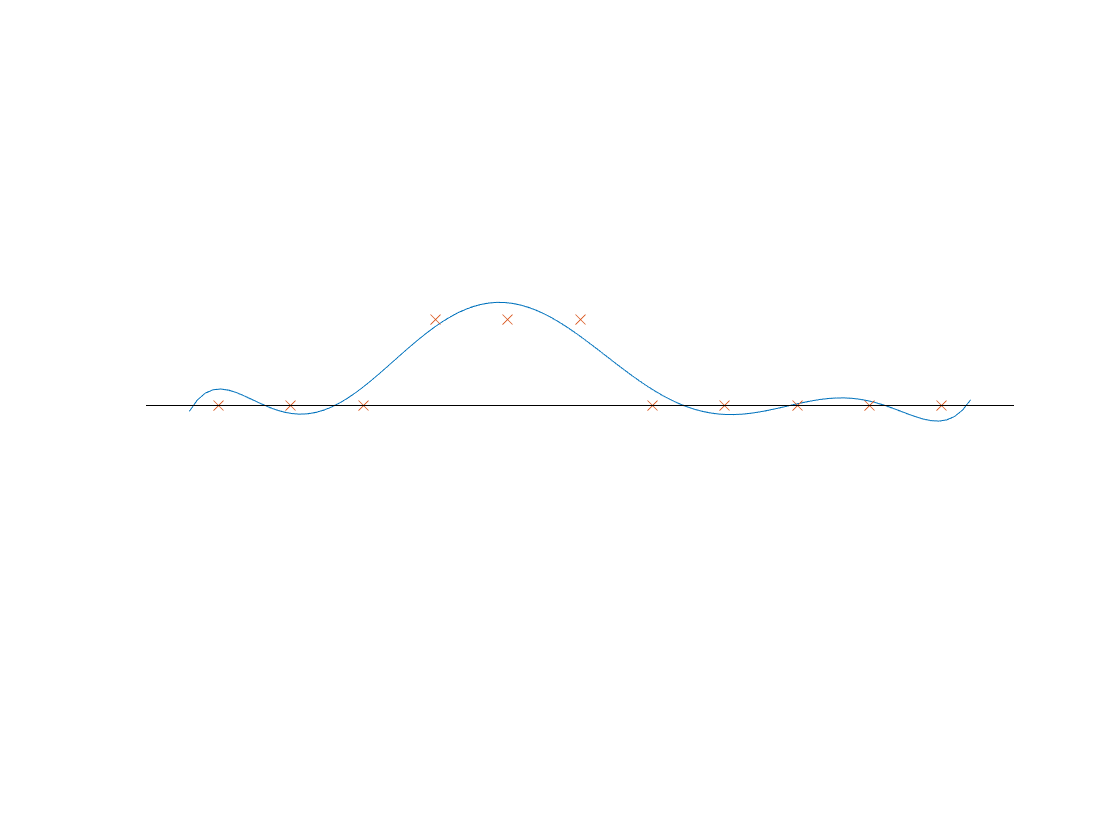
\includegraphics[width = \textwidth]{plot3.png}
    \end{center}
  \end{figure}



  
\end{exercise}












\begin{exercise}{P17} How closely, as measured in the $L^2$ norm on the interval $[1, 2]$ can the function 
  $f(x) = x^{-1}$ be fitted by a linear combination of the functions $e^x$, $cos(x)$, and $\sqrt{x}$? Write 
  a program that determines the answer to at least two digit of relative accuracy using a discretization of $[1, 2]$
  and a discrete least squares problem. Write down your estimate of the error and also of the coefficients of 
  the optimal linear combination, and produce a plot showing both $f(x)$ and the optimal approximation.\\
  \solution Using MATLAB to fit the function we get the following function, a maximum residual of $\approx .038$
  and an accuracy under the $L^2$ norm of $\approx .0105$,
  \begin{equation*}
    F(x) = 0.1521e^x +  1.1758\cos{x} - 0.0794\sqrt{x}
  \end{equation*}
  \textbf{Console:}
  \begin{center}
    \lstinputlisting[basicstyle = \small]{r3.txt}
  \end{center} 
    \begin{figure}[H]
      \begin{center}
        \caption{Plot of $f(x)$ and Best Approximation}
      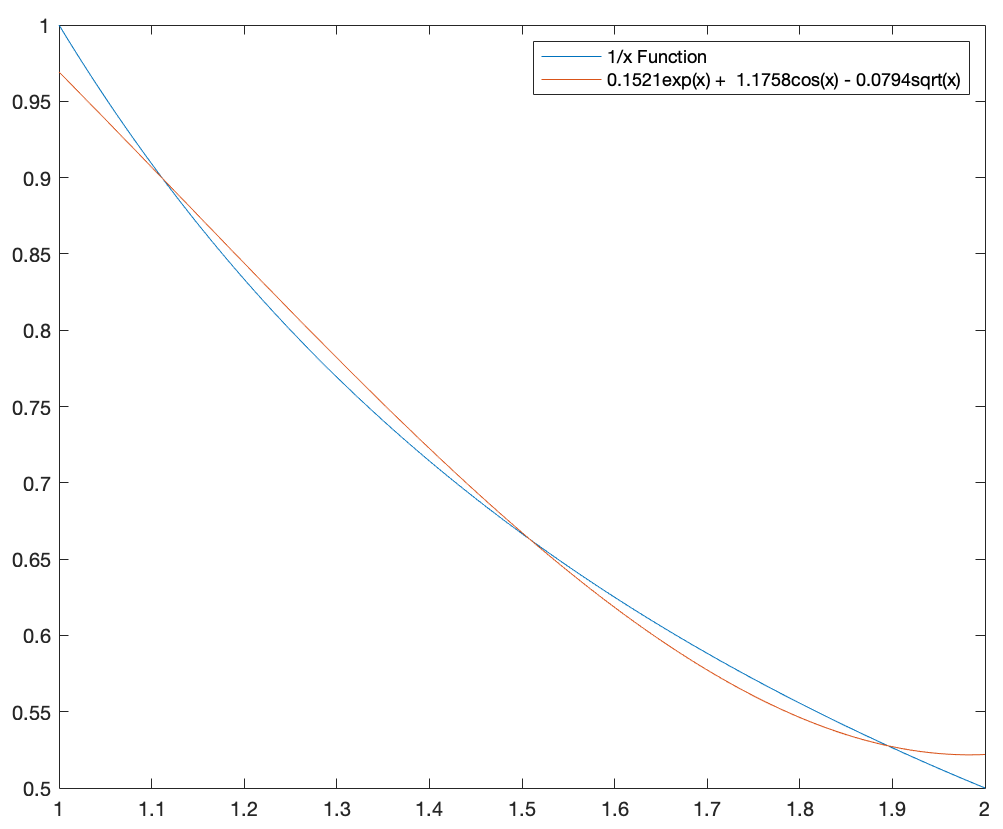
\includegraphics[width = .85\textwidth]{plot.png}
      \end{center}
    \end{figure}
  


\end{exercise}


\vspace{1in}


%%%%%%%%%% Double check
\begin{exercise}{10.1} Determine the (a.)eigenvalues, (b.)determinant, and (c)singular values of a householder reflector, 
  For the eigenvalues, give a geometric argument, as well as an algebraic proof.\\
  \begin{enumerate}
    \item[a.] Recall that a Householder reflector $F$ is defined by $F = I - 2P$ where $P$ is some orthogonal projector.
    Recall that in P12 we showed that projectors have eigenvalues of either $1$ or $0$. Furthermore, by Theorem 6.1 (equation 6.5) when an orthogonal projector is formed by 
    a single vector outer-product, like in $F$ we know that, 
    \begin{align*}
      P &=  Q\Lambda Q^*\\
        &\begin{bmatrix}
          \vert & \vert & \vert & \dots\\
          v     & q_1     & q_2 & \dots\\
          \vert & \vert & \vert & \dots
      \end{bmatrix}
        \begin{bmatrix} 
         1 & \dots & \dots & \dots \\
         \vdots & 0 & \dots & \dots \\
         \vdots & \vdots & \ddots & \\
         \vdots&\vdots &        & 0 
      \end{bmatrix}
      \begin{bmatrix}
        \vert & \vert & \vert& \dots \\
        v     & q_1     & q_2& \dots  \\
        \vert & \vert & \vert& \dots
    \end{bmatrix}^*.
    \end{align*} 
    Suppose P has the following eigenvalue decomposition, $P =  Q^*\Lambda Q$. Let $I =   Q^* Q$ and note that by substitution we get, 
    \begin{equation*}
      F = I - 2P =  Q^* Q - 2 Q^*\Lambda  Q =   Q^*(I - 2\Lambda) Q.
    \end{equation*}
    Consider $I - 2\Lambda$ and note that by substitution $\lambda_1 = -1$ and $\lambda_{>1} = 1$ .\\
    Consider Figure 10.2. It shows how a vector $x$ is transformed under two possible reflectors $F$ based on choice of $P$ (or $v$) via the 
    addition of $v = ||x||e_1 - x$. Suppose we had some vector $x$ which lies in the output space of $F$. By definition $x$ must 
    be of the form $||x||e_1$, and therefore when passed through $F$ again we must get the same vector since $v = ||x||e_1 - x$. When $v$ is defined 
    by $v = -||x||e_1 - x$ we get the similar $\lambda_1 = -1$ case. 
    \vspace{.15in}

    \item[b.] From the previous problem we found an eigenvalue decomposition of $F =  Q^*(I - 2\Lambda) Q$. Applying the determinant we get, 
    \begin{equation*}
      det(F) = det( Q^*(I - 2\Lambda) Q) = det(Q^*)det(I - 2\Lambda)det(Q) = 1*-1*1 = -1.
    \end{equation*}  

    \vspace{.15in}
    \item[c.] For the singular values of $F$ simply consider the eigenvalue decomposition from part a. Taking the absolute value of the $I - 2\Lambda$ term
    and adjusting $Q$ accordingly we get an SVD where the singular values are all $\sigma = 1$.
  




  \end{enumerate}
\end{exercise}


\vspace{1in}


\begin{exercise}{10.2}
  \begin{enumerate}
    \item[a.] Write a Matlab function $[W,R] = house(A)$ that computes an implicit representation of a full $QR$ factorization 
    $A = QR$ of an $mxn$ matrix $A$ with $m \geq n$ using Householder reflections. The output variables are the lower-triangular matrix
    $W \in \CC^{mxn}$ whose columns are the vectors $v_k$ defining the successive Householder reflections, and a triangular matrix $R \in \CC^{n,n}$\\
    \solution Consider the following Matlab function,\\
    \textbf{Code:}
  \begin{center}
    \lstinputlisting[basicstyle = \small]{r4.txt}
  \end{center} 
  \textbf{Console:}
  \begin{center}
    \lstinputlisting[basicstyle = \small]{r5.txt}
  \end{center} 
    \vspace{.5in}


    \item[b.] Write a Matlab function $Q = formQ(W)$ that takes the matrix $W$ produced by $house()$ as input and 
    generates a corresponding $mxm$ orthogonal matrix $Q$.\\
    \solution Consider the following Matlab function,\\
    \textbf{Code:}
    \begin{center}
    \lstinputlisting[basicstyle = \small]{r6.txt}
    \end{center} 
    \textbf{Console:}
    \begin{center}
      \lstinputlisting[basicstyle = \small]{r7.txt}
    \end{center} 
      \vspace{.5in}
  \end{enumerate}
\end{exercise}
\vspace{1in}
  

\begin{exercise}{11.3} Take $m = 50$, $n = 12$. Using Matlabs's linspace, define $t$ to be the $m$-vector corresponding to linearly spaced 
  grid points from 0 to 1. Using Matlab's vander and fliplr, define $A$ to be the $mxn$ matrix associated with least squares fitting on this 
  grind by a polynomial of degree $n-1$. Take $b$ to be the function $\cos(4t)$ evaluated on the grid. Now calculate and print( to 16 digit
  precision) the least squares coefficients vector $x$ by six methods: 
  \begin{enumerate}
    \item[a-f.] Compare the various algorithims used to solve least squares problems.\\
    \solution Consider the following Matlab script.\\
    \textbf{Code:}
    \begin{center}
    \lstinputlisting[basicstyle = \small]{r8.txt}
    \end{center} 
    \begin{center}
    \lstinputlisting[basicstyle = \tiny]{r9.txt}
    \end{center} 
    The scripts computes the least squares coefficient for a degree 11 polynomial approximating the function 
    $\cos(x)$ on the interval $[0, 1]$ with 50 equally spaced points. Each column represents the coefficients in ascending order of one solving method
    in the order they where computed ie. column 6 was computed via SVD. \\
    \vspace{.15in}

    \item[g.] The calculations above will produce six lists of twelve coefficient. In each list, highlight the digits that appear 
    wrong, Comment on what differences you observe. Do the normal equations exhibit instability? You do not have to explain your observations.\\
    \solution Consider the solutions given from the previous Matlab script. In our discussion of these algorithms we concluded that the SVD is the most stable algorithm, in comparing each algorithm I used 
    the SVD as the baseline/true answer. We can see that the Normal Equations method seems to produce the most
    rounding error.  
    \begin{figure}[H]
      \begin{center}
      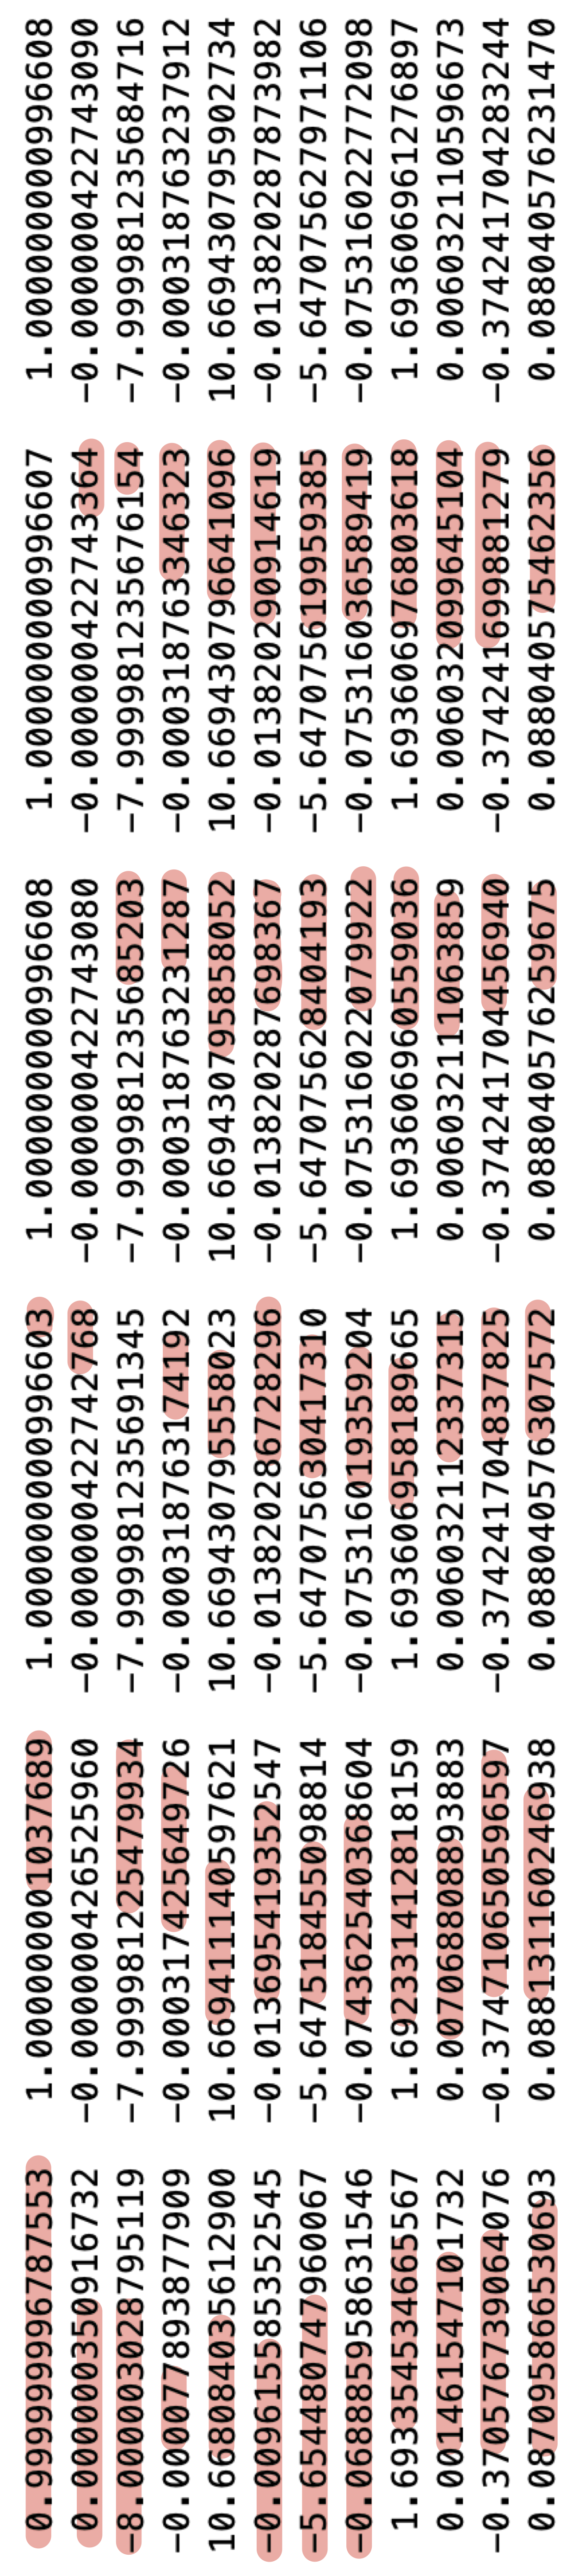
\includegraphics[width = .33\textwidth]{plot1.png}
      \end{center}
    \end{figure}



    
  \end{enumerate}
  
\end{exercise}


\end{document}






























